\documentclass[11pt]{article}

\usepackage{amsmath}
\usepackage{amsfonts} % to include additional math. characters such as R
\usepackage{graphicx} % to include images
\usepackage{hyperref} % to be able to click on references
\usepackage{multirow} % to merge cells in tabular env. vertically
\usepackage{subcaption} % for subfigures and +
\usepackage{longtable} % to have table that extends over multiple pages
\usepackage{lipsum}
\usepackage{color}
\usepackage[parfill]{parskip}
\usepackage[thinc]{esdiff} % for easier d/dx commands
\usepackage[left=2cm, right=2cm, bottom=3cm, top=3cm]{geometry}

% Additional commands
\newcommand*\dif{\mathop{}\!\mathrm{d}}

\graphicspath{ {./Images} }
\title{Cancer Immunotherapy - Planning Report}
\author{Alexandre Y. Péré }
\date{\today}

% What does not count: title page, table of content, abstract, acknowledg.
% tables and figures, appendices, captions, nomenclature and biblio.
% So what counts: section pure content
\begin{document}
\begin{titlepage}
    \newcommand{\HRule}{\rule{\linewidth}{0.5mm}}
    \begin{center}
        \HRule \\[0.4cm]
    { \LARGE \bfseries Bayesian Modelling to Characterise the Responder Profile to a  Novel Cancer Immunotherapy\\[0.55cm] }
    { \large Supervisors: Professor Reiko Tanaka, Doctor Tara Hameed} \\
    v2.2
    \\[0.4cm]
    \HRule \\[0.5cm]
    { \large Alexandre Yann Péré \\[0.1cm]
    CID: 01938104  \\[0.1cm]
    \today \\ [0.1cm]
    \vspace{10pt}
    Word Count: 4148}
    \end{center}
\end{titlepage}

\tableofcontents


% Repartition of word count (total 4,000)
%
% Project specification (300)
% Litt Review (1,200-1,500)
% Schedule (500)
% Evaluation (300)
% Prelim Results (1,000)
% total=3,000

% QUESTIONS FOR TARA
% 1) What's the difference between GA validation and Bayesian validation??
\pagebreak 
\section{Project Specification}\label{sec:specs}
% This section should state clearly what the project is intended to deliver. It should contain the AIMS, OBJECTIVES and HYPOTHESES of your work.

% Questions/comment: 
% - Should include "optimisation of treament for CR" in aims?
\subsection{Background}
\subsubsection{Cancer}
Cancer is a large class of diseases that is the second leading cause of death in the United-States \cite{nchs}. While the immune system has the potential to target and eliminate cancer cells, cancer often finds ways to evade these natural defenses \cite{EvasionMech}. Traditional methods, such as chemotherapy or surgery, rely on using destructive external agents to kill the cancerous cells. However, introducing foreign agents in the body often results in heavy side effects \cite{oncologyTreatRev}. This prompted the development of immunotherapies, a type of treatment aimed at countering cancer's ability to escape immune detection, which thus has the potential to be less toxic. Several viable strategies exist for immunotherapy \cite{ReviewCPI}. We will first review the general principles behind these stratgeies.

\subsubsection{Immunotherapies}
\textit{Cytokine-based Therapies}\\[3pt]
Cytokine-based therapies rely on the injection of specific cytokines (small proteins that act as signalling molecules during the immune response) to control tumour growth \cite{ioDef}. One of the most promising cytokine thus far is the interleukin-12 (IL-12), that was shown to have potent antitumour effects \cite{il12IsCool}. While it does not directly affect tumour cells, it mediates the production of other molecules or cells that have a more direct effect \cite{il12CytokineStorm}. First of all, it activates the production of tumour-infiltrating cytotoxic cells, mainly CD8$^+$~\cite{cd8FirstWay}. These are a type of T-lymphocytes whose main function is to carry out cytotoxic activity (i.e. killing the malignant cells) after detecting tumoural antigen~\cite{cd8Effects}. Secondly, they induce production of another type of cytokine, called interferon-$\gamma$ (IFN$\gamma$) \cite{ifnIL12}. IFN$\gamma$ in turn affects the tumour microenvironment by stimulating production of cytotoxic cells \cite{ifngNKProd}, reducing angiogenesis \cite{ifngAngiogenesis} and upregulating antigen-presenting pathways within tumour cells \cite{ifngAntigenExposure}. Lastly, IL-12 facilitates T-cell proliferation (including CD8$^+$) by reducing negative regulatory pathways that lead to immunosuppression \cite{reducImmunoSuppression}. It does so by inhibiting the effect of immune checkpoint Programmed Death 1 (PD1), following a similar strategy to checkpoint inhibitor (CPI) treatments. While these three pathways indicate that IL-12 has a very robust antitumour effect, clinical studies demonstrated that systemic injection of IL-12 is exceedingly toxic as it triggers a large immune response throughout the whole body \cite{clintriAC1}\cite{clintriAC2}. These severe treatment-related adverse effects (TRAEs) dampened research about IL-12, waiting for a safer, more localised delivery method to be found.\\[12pt]
%
\noindent\textit{Immune Checkpoint Inhibitors}\\[3pt]
The usual partner of cytokine-based treatments are checkpoint inhibitors. To understand checkpoint inhibition, we must first review in more detail the negative regulatory pathways of CD8$^+$ T-cells activity. The most potent pathway involves checkpoint molecules, either Cytotoxic T-lymphocyte antigen 4 (CTLA4) or programmed cell death 1 (PD1) \cite{cpiProof}. Both molecules are membrane protein receptors that act with some delay to exhaust and deactivate T-cell functions after they are stimulated by antigen-presenting cells (APC). Both CTLA4 and PD1 function in similar ways, the main difference being the type of tissues they affect \cite{PDvsCTLA}. Although their original function was shown to be prevention of autoimmunity \cite{PD1Autoimmune}, they lead to immunosuppression in the presence of tumours. The idea behind CPI treatments is to inhibit these regulators to shift the tumour microenvironment away from immunosuppression. Clinical trials demonstrated positive results in several types of cancers , but performed poorly against immunologically cold tumours, i.e. tumour that do not normally elicit a strong immune response (they escape the immune system very effectively), such as melanoma \cite{antiCTLA4Mel}.

% \subsection{Experimental Data}
% Add data plots here.
\subsection{Previous Work on Computational Modelling}\label{ssec:prevWork}

To have a better understanding of the immune response to the treatment, T. Miyano, 2019 \cite{takuya}, proposed to use a computational modelling approach. Computational models are common in pharmacodynamics as they can be analysed with mathematical tools, potentially revealing key mechanisms to optimise the treatment. He developped an initial mechanistic model based on Delay-Differential Equations (DDEs), parameterised by 21 parameters representing various relevant biological factors of a given mouse, such as the tumour growth rate or the degradation rate of IFN$\gamma$ \cite{takuya}: 
\begin{align*}
    \dot{g}(t) &= k_1 + k_2 [d_{CBD}(t) + d_{12}(t)] - d_1g(t) \\ 
    \dot{c}(t,t-t_d) &= k_3 + k_4g(t-t_d)-d_2c(t) \\ 
    \dot{p}(t) &= k_5 - [d_3 + d_4g(t)]p(t) \\ 
    \dot{v}_l(t) &= k_6\left[1 - \frac{v(t)}{v_{max}} \right]v_l(t) - \left[d_5 + \frac{\frac{d_6c(t)}{1+s_1p(t)(1-d_{CPI}(t))}+d_7g(t)}{1+s_2v(t)}\right]v_l(t)\\
    \dot{v}_d(t) &= \left[d_5 + \frac{\frac{d_6c(t)}{1+s_1p(t)(1-d_{CPI}(t))}+d_7g(t)}{1+s_2v(t)}\right]v_l(t) - d_8 v_d(t)
\end{align*}
The five state variables ($g$, $c$, $p$, $v_l$ and $v_d$) are concentration of IFN$\gamma$, of CD8$^+$ and of PD1 along with volume of living and dead tumour, respectively. This was motivated by the fact that these are the key players in the immune response, as explained above. The meaning of each parameter is reported in the Appendix. The model was investigated by C. Hines, who showed that the model could successfuly reproduce experimental data by using a Genetic Algorithm for parameter fitting \cite{christian1}. However, C. Hines also demonstrated in a subsequent analysis that the model had \textcolor[rgb]{0.7,0.2,0.2}{[significant differences]} with findings from the biologists in two ways. A positive feedback loop, where IL-12-induced IFN$\gamma$ in turn produces IL-12, is missing from the model \cite{christian2}. Additionally, C. Hines showed that the model outcome does not depend much on the initial tumour volume and treatment characteristics (day of injection, number of doses, etc.)\cite{christian1}, which is opposite to results reported in \cite{cbdil12}. Rather, he found that the model depends almost exclusively on parameter $k_6$, $d_1$ and $s_2$ (which respectively corresponds to proliferation rate of tumour; degradation rate of IFN$\gamma$ and tumour-induced immunosuppression strength)

\subsection{Motivation}

\par Recent endeavours in this field of immunotherapies led to the development by Ishihara group at Imperial College in 2019 \cite{cbdil12} of a new molecule, CBD-IL-12, that demonstrated promising results to treat melanoma. The CBD-IL-12  molecule consists of a collagen-binding protein (or collagen-binding domain, CBD) that is fused onto a IL-12 cytokine. The modified interleukin hence mainly accumulates in collagen-rich regions. As collagen is the main component of cancerous microenvironment \cite{collagenInCancer}, this effectively results in an enhanced delivery method that can achieve high concentration of IL-12 specifically in cancerous microenvironments. In mice tumour-models, this novel molecule achieved a CR \textcolor[rgb]{0.7,0.2,0.2}{[must explain CR rate]} rate of up to 67\% ($n=15$) for melanoma, and 87\% ($n=15$) for breast cancer when combined with CPI drugs (a mix of both anti-PD1 and anti-CTLA4). While these results are encouraging, the study showed that such high CR-rates could only be achieved in very specific settings (such as a tumour volume of 70mm$^3$ upon injection \textcolor[rgb]{0.7,0.2,0.2}{[add details]}). Different settings (e.g. volume of 150mm$^3$) elicited little to no response. This heterogeneity of treatment outcome could not be explained by the authors. The first step to improve efficacy of CBD-IL-12-based treaments would thus be to understand better what are the key parameters that control the treatment outcome. 

As outlined above, the aim of the project is to identify biological factors involved in the immune response that determine treatment outcome (CR vs non-CR), along with their critical value that lead to a bifurcation. These biological factors correspond to the parameter of the DDE model. However, the first key issue is that these parameters are kinetic rates that cannot be measured experimentally. We thus have to estimate them solely from the measurable data (i.e., tumour volume). This process is called parameter estimation. The other key challenge is that the data collected concerns multiple mice drawn from the same population. There is hence some shared information between the mice, as well as some variability between that explain the range of output obtained in the lab. Nonlinear mixed-effects models \cite{Davidian2011} are a standard method to analyse population dataset with both shared information (called fixed-effects) and individual variability (called random-effects).

\subsection{Aims and Objectives}
\noindent The aim of this project is to use computational models to improve our understanding of the immune mechanisms behind the CBD-IL-12 immunotherapy, utlimately to characterise the responder profile for the treatment.\\[8pt]
\textbf{Objective 1:} change the initial mechanistic model to a mixed-effect model so that it can reproduce the experimental data while including all the important pathways of the immune response.\\ 
\textbf{Objective 2:} analyse the mixed-effect model to identify key biological factors in mice that determine the outcome of the treatment, along with the corresponding threshold that separates complete response (CR) from non-CR 
% \textbf{Objective 3:} associate key factors to potential biomarkers in mice\\ 
% \textbf{Objective 3:} understand how the boundary between CR and non-CR depends on the treatment characteristics (number and frequency of doses, combination with other treaments, etc.)

\section{Ethical Analysis}
%This should be a short section. Mention the ethical basis, background, and implications of the project regarding subjects and specimens used and their provenance, data derived or measured and their use. Include the long-term effects and meaning of the work, as well as the effects of the work on colleagues, the College, society and the environment as appropriate.

Treatments and experiments on the specimens used, mice in this case, were approved by the Institutional Animal Care and Use Committee of the Univerity of Chicago (see Methods section of \cite{cbdil12}).

The data derived from these experiments holds immense potential for understanding treatment response in cancer, aiding in the optimization of therapies for human use.

Long-term implications involve the potential for groundbreaking advancements in cancer treatment, benefiting society globally. However, considerations extend beyond treatment efficacy to encompass environmental impact, fostering sustainable practices in research, and ethical ownership and dissemination of findings. Collaboration among colleagues, stakeholders, and the wider community fosters responsible research conduct and knowledge dissemination while ensuring transparency and accountability. Additionally, financial sustainability and social responsibility in implementing these therapies for public benefit are essential considerations.

To ensure that the results are true and reliable, the full analysis along with the code will be published on GitHub.
% \pagebreak

\section{Literature Review}\label{sec:littrev}
% Summarise the key findings from a range of published sources that you have used to identify research gaps, shape your aims and objectives, and justify the decisions you are making in your methodology. The text should be clear, with use of figures (with attribution) if helpful to the explanation.

In this section we will give an overview of the mathematical tools relevant for the project that were mentioned in Section~\ref{sec:specs}. Starting by presenting the process of parameter estimation, we will then focus specifically on the general Bayesian method and extend it its hierarchical version.  

\subsection{Overview of Parameter Estimation}
Since the model developed by Miyano is based of DDE, we will focus in the followings sections on DDEs. Let the general definition of a DDE model be: 

\begin{align*}
    \diff{X_i}{t} = f_i(t, \boldsymbol{X}(t), \boldsymbol{X}(t-\tau)| \boldsymbol{\theta}), \qquad t \in [t_0, t_{max}], i = 1, \ldots, I
\end{align*}

where $\tau$ denotes a constant delay, so that the rate of change of state $X_i$ depends on both the present state $\boldsymbol{X}(t)$ and a past state $\boldsymbol{X}(t-\tau)$. The subscript \textit{i} indexes the different state variables of interest, and $\boldsymbol{\theta}$ is the (unknown) vector of the parameters for the DDE model. This parameter vector is different for each treated mouse, as it uniquely characterises its treatement response, and hence we denote with $\boldsymbol{\theta}_j$ the parameter vector that characterises the $j$-th mouse. The experimentally observed tumour evolution for the $j$-th mouse is denoted by $\boldsymbol{y}_j$, and each of its elements is the tumour volume observed at a given time, noted $y_{j}(t)$. The aim of parameter estimation is to retrieve the parameter vector that can reproduce the observed data. Mathematically, this can be expressed as maximising the likelihood of the observations $\mathcal{L}(\theta;\boldsymbol{y})$, where $\eta_j$ is the random effect for individual $j$ \cite{SAEM}. 
\begin{align*}
    \mathcal{L}(\boldsymbol{\theta};\boldsymbol{y})=\prod_{j} \mathcal{L}(\theta;\boldsymbol{y}_j)=\prod_j p(\boldsymbol{y}_j\vert \boldsymbol{\theta})=\prod_j \int p(\boldsymbol{y}_j\vert \eta_i,\boldsymbol{\theta})p(\eta_j\vert \boldsymbol{\theta}) \,d\eta_j
\end{align*}

Many statistical approaches have been developed to perform parameter estimation on differential equation models from noisy data \cite{liu_wang}. However, most of them cannot be applied to mixed-effect models. In the context of pharmacodynamics model , Donnet et al, 2013 \cite{revParamEst} reviewed different techniques available to perform parameter estimation. For analysis of population data with observational noise, two methods are available: Expectation-Maximisation (either Stochastic \cite{SAEM} or using First-Order Condition \cite{foce} (FOCE)) and Bayesian parameter estimation \cite{rosenbaum}. The authors concluded that Bayesian modelling in particular is the most flexible method, since it does not rely on assumptions and hence work both inidividual or population datasets, with or without noise, which is not the case for alternative methods. Additionally, it benefits from theoretical validity although at the cost of being more computationally intensive, whereas the FOCE method was not proven to converge to the true posterior. Another relevant advantage is that Bayesian approach do not provide point estimate, but rather distributions, which could be key to explain outcome heterogeneity. Hence the Bayesian modelling approach seems to be the most relevant for the project. 

\subsection{Bayesian Parameter Estimation}

Bayesian Parameter Estimation is a method to estimate $\boldsymbol{\theta}_j$ given an observation vector $\boldsymbol{y}_j$. Contrary to frequentist approach, estimations are in the form of probability distributions (called posteriors, denoted $p(\boldsymbol{\theta}|\boldsymbol{y})$) rather than point estimates. 

For a situation where data about only one individual was gathered, the posterior distribution is defined as follows \cite{tbk_gelman}:
\begin{align*}
    p(\boldsymbol{\theta} | \boldsymbol{y}) \propto p(\boldsymbol{\theta})p(\boldsymbol{y}|\boldsymbol{\theta})
\end{align*} 
This formula is the direct application of Bayes' theorem. It is the product of the prior distribution $p(\boldsymbol{\theta})$, which represents our knownledge of the problem, and the likelihood $p(\boldsymbol{y} | \boldsymbol{\theta})$. Before further defining these distributions, we must extend this definition of the posterior distribution to work for mixed-effect models, called hierarchical models in Bayesian statistics. 

\subsection{Hierarchical Modelling}
We seek to estimate the probability distribution of the parameter vector $\boldsymbol{\theta}$ for each individual, however these vectors are not independent from each other since each individual is sampled from a common population (mixed-effect model). To analyse mixed-effect model, hierarchical Bayesian modelling is a standard method \cite{revParamEst}\cite{rosenbaum}. For example, Rosenbaum et al., 2019 \cite{rosenbaum}, studied models of predator-prey systems, which also display radically different behaviours depending on the values of certain kinetic rates that cannot be directly measured. By fitting times series of measurable data to a hierarchical Bayesian model, they could not only extract a specific set of parameters for each individual system; but also determine the regions in parameter space that led to radically different types of behaviour accross the population. As this study present many similarities with the current project, it shows that hierarchical Bayesian modelling is a promising tool that is worth exploring.

Hierarchical modelling enables us to formulate that the parameter vector $\boldsymbol{\theta}_j$ is sampled from an population-level distribution characterised by the (also unknown) hyperparameters $\boldsymbol{\phi}$. The objective is hence to find the distribution of both $\boldsymbol{\theta}_j~\forall j$ and $\boldsymbol{\phi}$. The Bayesian parameter estimation framework integrates this additional assumption by changing the posterior to \cite{tbk_gelman}:
\begin{align*}
    p(\boldsymbol{\theta}, \boldsymbol{\phi} | \boldsymbol{y}) \propto p(\boldsymbol{\phi})p(\boldsymbol{\theta}|\boldsymbol{\phi})p(\boldsymbol{y}|\boldsymbol{\theta})
\end{align*} 

This expression is a product of the hyperprior $p(\boldsymbol{\phi})$, the population distribution $p(\boldsymbol{\theta}|\boldsymbol{\phi})$ and the likelihood $p(\boldsymbol{y}|\boldsymbol{\theta})$.

\subsubsection{Hierarchical Priors and Hyperpriors}
In hierarchical Bayesian models, there are two types of parameters: hyperparameters $\boldsymbol{\phi}$ and individual parameters $\boldsymbol{\theta}_j$ \cite{tbk_gelman}. The key feature is that the simulated data is directly conditioned on the regular parameters, which are themselves drawn from population-level distributions characterised by hyperparameters. Hence, this results in two types of priors: hierarchical priors, that specify how to sample $\boldsymbol{\theta}$ using the hyperparameters $\boldsymbol{\phi}$; and hyperpriors that convery our knowledge about the potential values of~$\boldsymbol{\phi}$.

For the case of Bayesian parameter estimation on sets of time series, Rosenbaum et al, 2019 \cite{rosenbaum}, proposed to sample each ODE parameter from a Normal distribution. As Normal distribution are characterised by two values (mean $\mu$ and standard deviation $\sigma$), this resulted in two hyperparameters per ODE parameter. This can be summarised as follows, for a given scalar parameter $\theta$:
\begin{align*}
    \theta &\sim p(\theta | \phi) \Leftrightarrow \theta \sim \mathcal{N}(\phi_\mu, \phi_\sigma) \quad &&\textit{hierarchical prior} \\ 
    \phi_\mu &\sim p(\phi_\mu) \quad &&\textit{hyperprior for the hyper-mean} \\ 
    \phi_\mu &\sim p(\phi_\mu) \quad &&\textit{hyperprior for the hyper-standard deviation} 
\end{align*}
By adding additional hyperparameters, this definition could be modified to allow for bimodal distribution instead of a simple normal distribution for the hierarchical priors.

\subsubsection{Likelihood function}
The likelihood function in the Bayesian framework is how we model the dynamics of the underlying process. In pharmacodynamics, it is the mechanistic model of the immune response. Assuming that the observational noise is a white Gaussian noise with zero-mean and a standard deviation $\sigma_{err}$ that is common to all experiments, the likelihood can then be defined as follows \cite{liu_wang}, \cite{likelihood_2} (for a given tumour evolution $\boldsymbol{y}_j$):
\begin{align*}
    \mathcal{L}(\boldsymbol{\theta}_j) = \prod_{t=t_0}^{t_{max}} \frac{1}{\sigma_{err}} \exp\left(-\frac{(y_{j}(t) - Y_j(t|\boldsymbol{\theta}_j))^2}{2\sigma_{err}^2}\right)  
\end{align*}
Where $Y_j(t|\boldsymbol{\theta}_j)$ is the simulated time series using the DDE model parameterised by $\boldsymbol{\theta}_j$, $t$ is the time index for the time series and $\sigma_{err}$ is the experimental error. This is usually obtained by numerical methods. Without additional information about the measurement methods, this is the approach suggested by Rosenbaum et al \cite{rosenbaum}.

% \subsubsection{Calcultion of the Marginal Posterior Distributions}\label{ssec:post}
% Once the joint posterior distribution has been obtained, we can proceed to calculate the marginal probability densities for $\theta_j \forall j$ and for $\boldsymbol{\phi}$ \cite{tbk_gelman}.

% First, we calculate the joint posterior distribution conditional on each time series individually, ie:
% \begin{align*}
%     p(\theta_j,\phi|y_j) = p(\phi) \mathcal{B}(\theta_j|\phi) \mathcal{L}(\theta_j)
% \end{align*}

% We can then calculate each individual marginal probability density (ie. for each vector $\theta_j$) as:
% \begin{align*}
%     p(\theta_j|y_j) = \int p(\theta_j, \phi|y_j) \dif \phi 
% \end{align*}


To find the marginal posterior distribution for the hyperparameter vector $\boldsymbol{\phi}$, we can marginalise out $\theta$ by integrating over $\theta$ the full joint posterior distribution (ie. accross all time series):
\begin{align*}
    p(\phi|y) = \int \prod_{j=1}^{J} p(\theta_j, \phi|y_j) \dif \theta 
\end{align*}

\subsection{Reduction of the Computational Burden}
\subsubsection{Sensitivity Analysis}
As pharmacodynamics models can generally contain a high number of parameters, the Bayesian approach, which is computationally intensive \cite{revParamEst}, can result in intractable computations. To this end, Vasquez-Cruz et al, 2012 \cite{tomgro}, proposed a method to reduce the number of parameters in an ODE model. By taking the example of a crop growth ODE model with 17 parameters, they used a senstivity analysis (namely, eFAST and Sobol' method) to identify the most influencial parameters, and used these results to design a reduced model with only 7 free parameters. More specifically, they followed a procedure highlighted by Varela et al, 2010 [need paper], according to which parameters that account for less than 10\% of the total effects can be considered as fixed parameters. Then, using a parameter fitting algorithm, they were able to show that this reduced model could still replicate the experimental data with minimal error. Additionally, they showed that the two sensitivity analysis methods (eFAST and Sobol' methods) yield different results. Hence, to ensure that all the important parameters are detected, both methods should be used.

\subsubsection{High-performance Computational Methods}
As the estimation of the posterior distributions cannot be evaluated analytically, Luengo et al., 2020 \cite{MCMethods}, pointed out that Markov-Chains Monte Carlo approach to approximate the posterior is the only feasible approach in most applications. While many different MCMC methods exist \cite{ReviewMCMCAlgo}, it was shown by Nishio et al, 2019 \cite{NUTSvsHMCvsGibbs} that the No U-Turn Sampler (NUTS) led to lower skewness of the posterior and more decorrelated samples compared to the other two popular algorithms, Gibbs and Hamiltonian Monte Carlo samplers. However, traditional MCMC methods, including NUTS, can have convergence problem \cite{mcmcTrapped}. Since we hypothesised that the posterior distribution might be multimodal, we need also need a robust sampler for this case. Liu et al, 2018 \cite{liu_wang}, proposed a new sampler called Stochastic Approximation Monte Carlo (SAMC), which is based on the idea of partitioning the parameter space in a finite number of subspaces and forcing the algorithm to explore each subspace. By running the algorithm on a parameter estimation problem for an ODE model of predator-prey system (defined in \cite{fussmann}), they showed that SAMC could successfully retrieve the correct parameter value, while traditional MCMC methods such as the Metropolis-Hastings method were stuck in local modes.

\subsubsection{Transforms}
Another finding from the study of predator-prey systems \cite{rosenbaum} is that log-transformation of the residuals make the inference much more robust, resulting in faster convergence and more accurate posteriors. This changes the likelihood function to the following:
\begin{align*}
    \mathcal{L}(\boldsymbol{\theta}_j) = \prod_{t=t_0}^{t_{max}} \frac{1}{\sigma_{err}} \exp\left(-\frac{\lbrack\ln(y_{j}(t)) - \ln(Y_j(t|\boldsymbol{\theta}_j))\rbrack^2}{2\sigma_{err}^2}\right)  
\end{align*}

% Question for Tara: what if the revised mechanistic model does not capture the dual outcome that is initially present? Does that mean the model is wrong, or that the dual outcome is not exactly accurate?

% In light of the knowledge gathered through the litterature review presented above, the proposed plan to fulfill the 4 (3?) objectives is as follows.\\[12pt]
% %
% \noindent\textbf{Task 1.1 -- Evaluation of the initial model (already completed)}\\
% This includes numerical stability/bifurcation analysis and sensitivity analysis to find the boundary between CR and non-CR in parameter space. This step is necessary to understand to general design principles that guide the development of a mechanistic model, and can potentially reveal some of the model weaknesses that need to be addressed. The sensitivity analysis is also key to reduce the dimensionality of the problem, since the model is otherwise too large and would result in intractable computations.\\[12pt]
% %
% \noindent\textbf{Task 1.2 -- Non-hierarchical model validation (already completed)}\\ 
% The second step is to verify whether the model can be used to perform Bayesian inference, as this will be the core of the analysis. Following the procedure highlighted  in the \textit{Bayesian Workflow} paper by Gelman et al., 2020, \cite{gelman2020bayesian}, the validation consists of three main tests: prior predictive check, fake data check and posterior predictive check. In Task 1.2 we will focus on validating complete- and no-pooling models since they are the basic blocks that we will use in Task 1.3 to construct the full hierarchical model.\\[12pt]
% %
% The above validation procedure might fail in two ways : either the model cannot produce results (for example, the MCMC chains cannot explore the posterior distribution well), or it produces wrong results. For each outcome, we present below the steps we plan to take to overcome these.\\[12pt]
% %
% \noindent\textbf{Task 1.2a (fall-back 1) -- Validate using Approximate Bayesian Computation (2-3 weeks)}\\ 
% In the event that the MCMC chains do not converge, it would be due to the high complexity of the likelihood function (the mechanistic model of the immune response), a set of five Delayed Differential Equations that cannot be solved analytically. One way to reduce this complexity would be to use Approximate Bayesian Computation (ABC), which is a likelihood-free framework \cite{ABCtuber}. This approach is a  realitvely easy to implement method that prevents convergence problems, at the cost of slightly less exact results. \\[12pt]
% %
% \noindent\textbf{Task 1.2b (fall-back 2) -- Validate using simplified likelihood function (3 weeks)}\\
% As suggested in the \textit{Bayesian Workflow} paper \cite{gelman2020bayesian}, another method to solve convergence issues would be to simplify the likelihood function, for example by using ODEs instead of DDEs. This is an alternative to ABC, and would require more time to implement as we need to completely review the tumour model. However, contrary to ABC, it is still a traditional Bayesian inference and hence results in less approxmation errors, as highlighted by Robert et al, 2011 \cite{ABCerror}\\[12pt] 
% %
% \noindent\textbf{Task 1.2c (fall-back 3) -- Modify the model (1 month)}\\ 
% In the event that the inference can be run but produces wrong results, the most sensible approach would be to modify the Bayesian model. Care will be taken to ensure that all the key interactions during the immune response are correctly translated into the mechanistic model. The first missing pathway that we plan to implement is the positive feedback loop mentioned in Section~\ref{sec:littrev}. During this process, we expect to use a Genetic Algorithm for parameter fitting. This will be useful to test that the mechanistic model can reproduce the data, without having to resort to a full Bayesian inference, where many additional elements interact together and can make precise diagnostic harder. \\[12pt] 
% %
% \noindent\textbf{Task 1.3 -- Validation of the hierarchical model (3 weeks)}\\ 
% We will validate the hierarchical model once its two components are verified (no-pooling and complete-pooling models) through Task 1.2. It is still a Bayesian model, so we plan to follow the same validation procedure as above (including the fall-backs)\\[12pt]
% %
% \noindent\textbf{Task 2.1 -- Extensive numerial analysis of the compuational model (1-2 weeks)}\\ 
% This is the first set of analysis we plan to do on the validated model. This includes a eFAST sensitivity test, which enables us to reduce the dimensionality of the problem. This makes practical implementation of the subsequent analysis possible, while minimising the error we introduce. Following this, we will perform a stability analysis to evaluate the boundary surface in parameter space that separates CR from non-CR. We expect a grid-search analysis to be sufficient, since w are only concerned with the location of the bifurcation point.\\[12pt]
% %This is the first set of analysis we plan to do on the validated model. First we perform a sensitivity analysis, using the eFAST method as justified in Section~\ref{sec:background}. This is necessary to know if a given parameter should be set as a free or fixed parameter. This makes practical implementation of the subsequent analysis possible, while minimising the error we introduce. Then, we plan to perform a bifurcation analysis to evaluate the boundary surface in parameter space that separates CR from non-CR. We expect a grid-search bifurcation to be sufficient, since only trans-critical bifurcation can happen (Hopf would not make biological sense... ?). \\[12pt]
% %
% \noindent\textbf{Task 2.1a (fall-back 1) -- ?}\\ 
% (What happens if the model does not capture the bifurcation behaviour? Does it mean that the model is wrong?) \\[12pt]
% %
% \noindent\textbf{Task 2.2 -- Full Bayesian Inference (3 weeks)}\\ 
% In this step we perform a full hierarchical Bayesian inference and analyse the posterior distributions to find patterns that could explain data heterogeneity. It is still unclear what type of patterns it would be, but we suspect that the posterior distributions might be bimodal, which explains the bimodal treatment outcome. Bimodal posterior could reveal the bifurcation point between CR and non-CR, which is key for the next step. Task 2.1 ensures that such a bifurcation point exists. \\[12pt]
% %
% \noindent\textbf{Task 3 -- Biomarker Identification}\\ 
% Having identified the key parameters that encode the outcome heterogeneity along with their bifurcation point, we will link each of them to a corresponding mouse biomarker. We suspect that the exact methodology will depend on which parameters are selected for this step, but we propose to follow to general methodology for biomarkers identification presented in Section~\ref{sec:background}, relying on genomic data and statistical tools. We will also make use of the already-existing litterature about cancer biomarkers that measure potential response to therapy. \\[11pt]
% %
% \noindent\textbf{Task 3.a (fall-back 1) -- Collect genomic data}\\ 
% If genomic data is not available, means that we will have to collect it first. It is likely that the project will thus not be finishable, so will only be able to design computational/theoretical framework for biomarker identification without practical implementation.  

\section{Risk Register}
The main risks are : 

\begin{table}[!ht]
    \caption{Table of the different risks associated with the project's objectives}

    \label{tbl:hyperparams}
\begin{longtable}{|p{3.5cm}|p{2.3cm}|p{2.3cm}|p{8cm}|}
    \hline
    \textbf{Risk} & \textbf{Likelihood} & \textbf{Impact} & \textbf{Mitigation Strategy}\\
    \hline
    \endfirsthead
    \hline
    \textbf{Risk} & \textbf{Likelihood} & \textbf{Impact} & \textbf{Mitigatio Strategy}\\
    \hline
    \endhead
    \hline
    \multicolumn{4}{|r|}{\textit{Continued on next page}} \\
    \hline
    \endfoot
    \hline
\endlastfoot
        \hline
        MCMC chains do\newline not converge  & High & Very high & 
        Two alternative methods can be used in this case.
        \textbf{Approximate Bayesian Computations,} which is a approach that does not rely on a likelihood function. It is relatively easy to implement but introduces additional approximation error. \textbf{Model simplification}, an approach proposed in \cite{gelman2020bayesian}. It consists of simplifying the likelihood function, and does not introduce additional error.
        \\ \hline 
        Model does not\newline pass validation protocol& High & Very high & Modify the immune response model to ensure that all key interactions are translated in the mechanistic model. We especially plan to implement the positive feedback loop mentionned in Section~\ref{ssec:prevWork}. \\ \hline 
\end{longtable}
\end{table}
\section{Evaluation}\label{sec:eval}
Below we present a list of the key components of the cancer immunotherapy project, along with a way to verify that they function correctly.
%\textit{Mechanistic Model of the Immune Response}\\[3pt] % TODO: appendix ??
%Bayesian inference are computationally intensive operations, and can be hard to diagnose if they do not produce results as intended, since many components interact together. In this section we explain how we will evaluate a particular component of the full model, the mechanistic model. The mechanistic model must pass these tests before being used for the full hierarchical Bayesian inference.

%The performance of the mechanistic model can be assessed by two criteria. First of all, it should be able to reproduce the data obtained in the lab by Dr. Ishihara. Since this is not a hierarchical model, we propose to use a Genetic Algorithm (GA) to perform parameter fitting on individual time series, which is the method used by C. Hines in his research. This enables us to find a parameterisation of the model that leads to the best simulation, along with the Mean-Squared Error to the true data. This metric can be used to validate that the model can produce data close enough to the experimental time series. To assess the second criteria, we will use a sensitivity analysis. It enables us to check that the model is sensitive to the same quantity as shown in the lab [wording is terrible here, need to rephrase], for example to the treatment specification or to the initial tumour volume, which is not the case for the current one. \\[11pt]

\textit{Bayesian Model}\\[3pt]
To build and validate the Bayesian model, we will follow the Bayesian Workflow procedure outlined in \cite{gelman2020bayesian}. It consists of three different tests:
\begin{itemize}
    \item \textbf{Prior Predictive Check:} we sample 1,000 sets of parameter from the priors and simulate tumour growth for each of them. The 95\% credible interval of the resulting collection of time series should contain our expected range of curves we can expect. Evaluation of this step is mostly qualitative.
    \item \textbf{Fake Data Check:} we first need to generate a artificial dataset using known values of parameters, and then fit the Bayesian model to these fake datasets. By comparing the results of the model (i.e. the estimated parameter value in the form of the posterior distribution) to the true values, we can conclude whether the model can successfully perform parameter estimation or not. The approach proposed by Gelman et al. \cite{gelman2020bayesian} is to verify that the 95\% credible interval of the posterior includes the true parameter value. Additionally, another possible approach detailed in \cite{rosenbaum} involves substracting the true parameter value from the posterior. This results in a ``error'' distribution that should theoretically be zero-mean. 
    \item \textbf{Posterior Predictive Check:} this is analogous to the prior predictive check, except that parameter are drawn from the marginal posterior distributions instead of the prior distributions. This results in a collection of simulated time series. The 95\% credible interval should contain the experimental time series obtined in the lab. 
\end{itemize}
\textit{Convergence of the MCMC Chains}\\[3pt]
As mentioned above, convergence of the MCMC chains is a critical element that needs to be evaluated, as it reflects the quality of the approximation of the posterior distribution [cite T. Moins et al]. The most popular method to assess convergence is the potential scale factor reduction, usually termed $\hat{R}$, developed by Gelman et al., 1992 \cite{rhat}. It can be calculated as follows:
\begin{align*}
    \hat{R} &= \frac{m+1}{m}\frac{\hat{\sigma}^2_+}{W}-\frac{n-1}{mn} \\ 
    W &= \frac{1}{m(n-1)}\sum^m_{j=1}\sum^n_{t=1}(\psi_{jt}-\bar{\psi}_j)^2 
\end{align*}
Where $m$ is the number of chains used to explore the posterior in parallel, $n$ is their length, $\hat{\sigma}^2_+$ is the variance of the chain with the highest variance, $\psi_{jt}$ is the value of the $j$-th chain at the $t$-th iteration, and $\bar{\psi}_j$ the mean value of the $j$-th chain. The authors additional highlight that a value close to 1 usually indicates convergence, usually the criterion is $\hat{R}<1.05$ for convergence.

\textit{Responder Profile}\\[3pt]
Once the responder profile has been characterised, its accuracy can be evaluated by comparing the predicted treatment outcome against the true outcome on a new batch of cancerous mice. The procedure to inoculate skin cancer, inject the immunotherapy and measure tumour volume should be the same as defined in \cite{cbdil12} and \cite{takuya}. To be robust against all cases, only half of the batch of cancerous mice should be predicted as complete responder according to the responder profile. This ensures that we can collect data about the accuracy for both true positives and of true negatives.

\section{Preliminary Results}

\subsection{Numerical Analysis}
\subsubsection{Numerical Stability Analysis}

The very first aspect of Miyano's model that we wanted to verify was its ability to capture two specific treatment outcome: CR vs non-CR. As these behaviours can essentially be characterised by the fixed-points of the model (if the steady-state behaviour of the model converges to high values of tumour volume, it is a non-CR behaviour, and vice-versa. See definition in Section~\ref{sec:specs}). We opted for a grid-search stability analysis, meaning that we sample reguarly-spaced points in parameter space and classify them as either CR or non-CR. Fig.~\ref{fig:mcsa} shows the resuls of this analysis, where each axis of the cube corresponds to the value of a $k_6$, $s_2$ or $d_1$ respectively. A can be seen, there seem the be a clear boundary between the two response modes, with very little ``mixing''. This suggests that it would be possible to predict how a given patient would respond to the treatment, by knowning on which side of the boundary he is.

\begin{figure}[!ht]
    \centering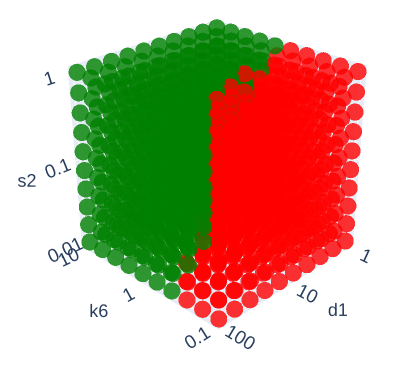
\includegraphics[scale=0.5]{stability.png}
    \caption{Stability analysis shows that there is a clear boundary in parameter space between CR and non-CR}
    \label{fig:mcsa}
\end{figure}

\subsubsection{Sensitivity Analysis}
In order to restrict the parameter space for subsequent analysis, and also to understand to main mechanisms behind the immune response, we performed a eFAST sensitivity analysis, which is a variance decomposition method. As it can only decompose variance of a scalar metric, it does not natively support time-series. Hence we chose to apply it to the integral of the tumour growth curve simulated by Miyano's model. This metric simply reflects the cumulative tumour volume over time, which is ultimately the quantity that we want to minimse. Other metrics which capture more specific feature of the tumour growth might be considered in the future, such as the derivative of tumour growth on the last simulated day to capture the patient's potential to go into CR. Results are shown in Fig.~\ref{fig:efast}. The total height of the bar represent the fraction of the variance that is imputable to the corresponding parameter. The first observation we can make is that model is mostly sensitive to $k_6$, $d_1$, $d_7$ and $s_2$. However, we can see that the main effect indices (in blue) are almost always negligible compared to the interaction indices (orange). According to a study by Vazquez-Cruz et al. (2012), this is a typical sign of non-identifiability \cite{tomgro} that will significantly hinder Bayesian inference. Additionally, results indicate that the treatment characteristics (labelled \verb+t_d+, \verb+t_delay+ and \verb+t_last+) have almost no impact on the treatment outcome, which is conflicting with the results experimentally obtained in the CBD-IL-12 study \cite{cbdil12}. Hence we suspect that the current model does not correctly model the immune response mechanisms. 

\begin{figure}[!ht]
    \centering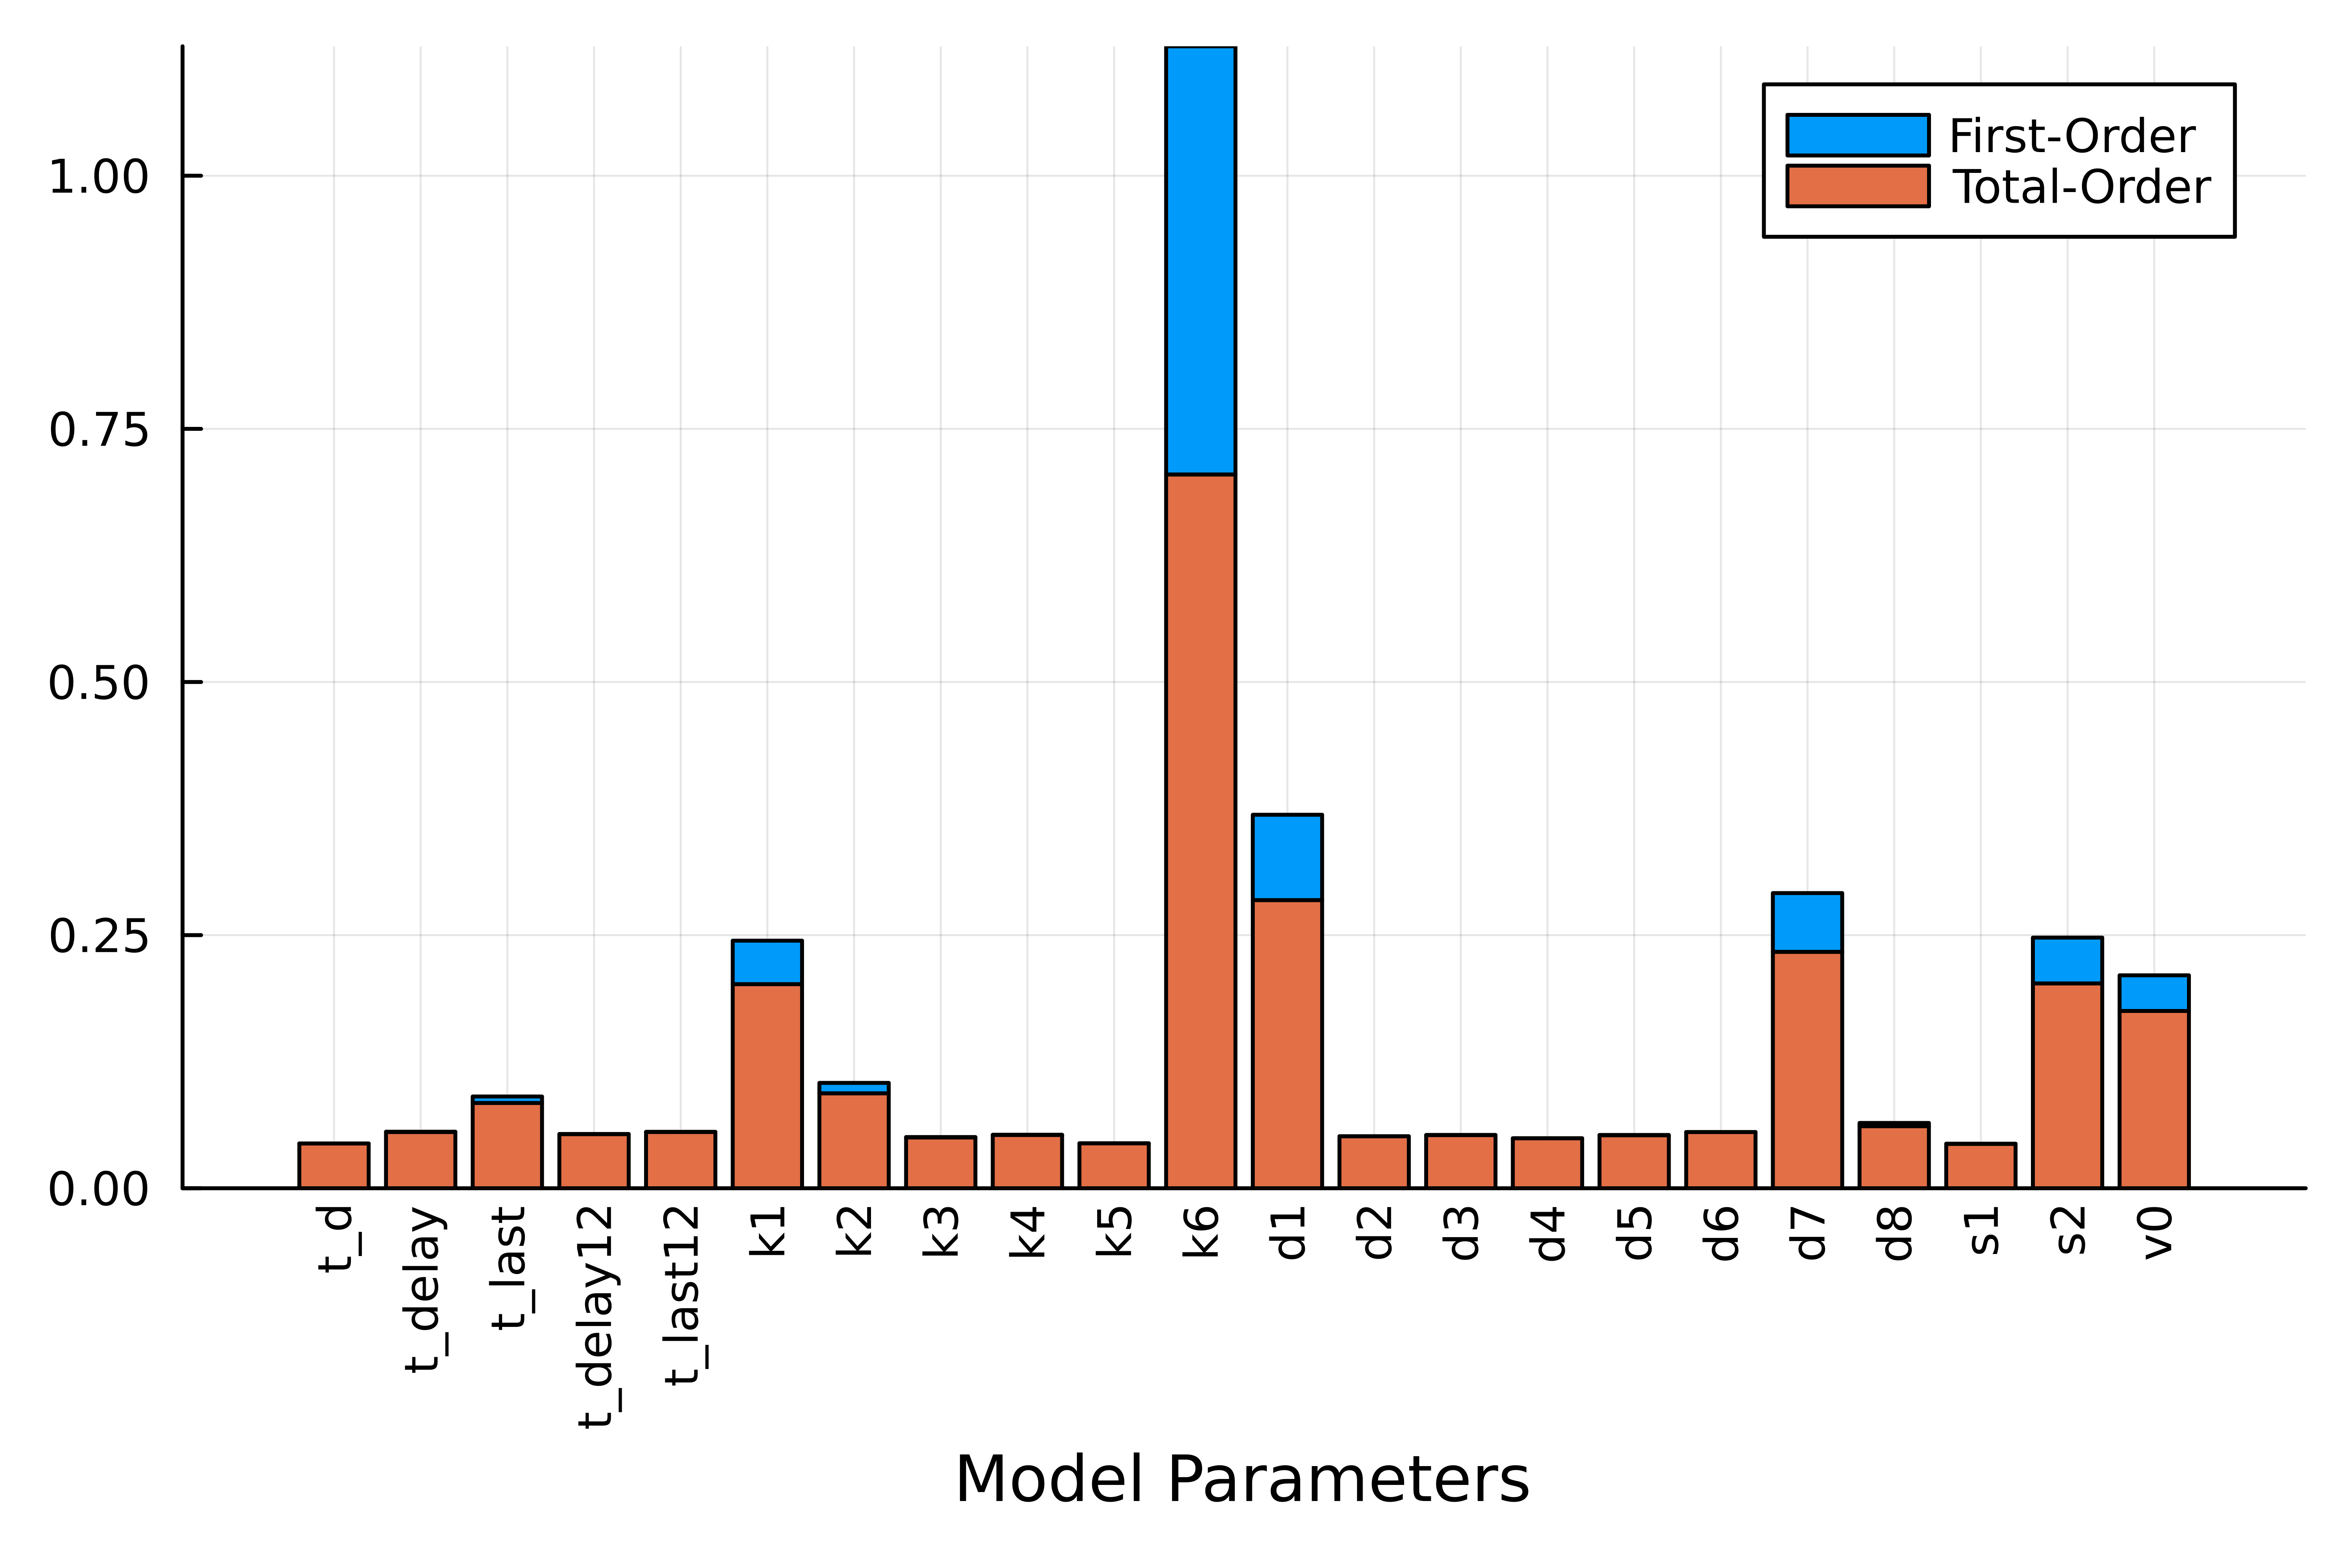
\includegraphics[scale=0.07]{proutiprouta.png}
    \caption{eFAST sensitivity analysis on Miyano's model shows that $k_6$ is the most influencial parameter by far, followed by $d_1$, $d_7$ and $s_2$. This is conflicting with findings from Ishihara group}
    \label{fig:efast}
\end{figure}

\subsection{Bayesian Model Validation}
In this section we show how the Bayesian model was validated, following the procedure highlighted in Section~\ref{sec:eval}. We focus on a reduced model with only three free parameters, $k_6$, $d_1$, $s_2$, which were identified by C.~Hines are the most impactful ones \cite{christian1}. All other parameters of the model were fixed to their respective value estimated by C. Hines to model the mean response curve. This ensures that each parameter is assigned a realistic yet arbitrary value.

\subsubsection{Prior Predictive Check}
In this case, we do not have much data on the typical values of the parameters since it is impossible to measure it (we only know that it is a positive number whose typical value is between 0 and 1, as evidenced by \cite{christian1}), so we aim to design an uninformative prior. Fig.~\ref{fig:ppc_1} shows a plot of 1,000 tumour growth time-series. Each of them was simulated using a set of parameters drawn from the following prior distribution:
\begin{align*}
    \ln(k_6) \sim \text{Cauchy}^-(0, 1) \\ 
    \ln(d_1) \sim \text{Cauchy}^+(0, 1) \\ 
    \ln(s_2) \sim \text{Cauchy}^-(0, 1) \\ 
\end{align*} 
We chose Cauchy distributions since that carry less information that standard Gaussian distributions, allowing for value far from their center of mass. This is critical since we do not have information about the true values of the parameters. As we exponentiate the Cauchy distribution, it means that $0 < k_6 < 1$. The blue shade represents the 95\% credible interval, and the dark green line is the median growth curve. As we can see, the 95\% credible interval is can virtually contain our expected range of curves, since it ranges from 0 (minimum volume) to 600 (maximum possible volume according to the equation), meaning that they are relatively uninformative priors. The median curve has the shape of the typical growth curve, as observed in the labs. Hence, we can say that the prior distribution is satisfying, as it could explain any potential growth curve while restricting the values of the parameters to a smaller subset of $\mathbb{R}$.
    \begin{figure}[!ht]
        \centering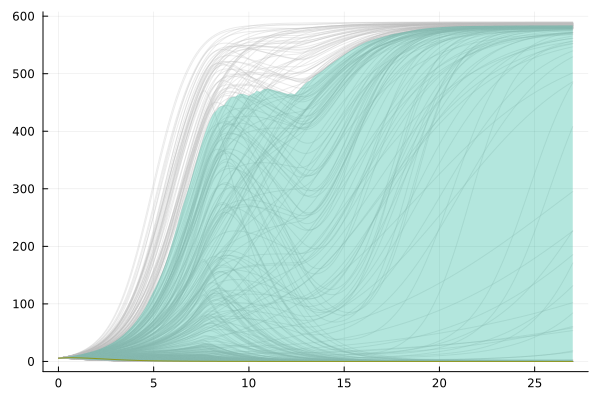
\includegraphics[scale=0.4]{model_validation/prout1.png}
        \caption{ODE solution for 1,000 parameter values sampled from the prior ($\boldsymbol{\theta} \in \mathbb{R}^1$)}
        \label{fig:ppc_1}
    \end{figure}

\subsubsection{Fake Data Check}
Each fake growth curve was generated by sampling a value of $\theta$ from the prior distribution, and then simulating the tumour growth in the same way as for the Prior Predictive Check. However, as biological data is always noisy, we also added some noise to make the fake dataset closer to what we would actually expect from the labs. This was done in two different ways, resulting in two distinct datasets. For dataset~A, we simply added a white standard Gaussian noise to the simulation. For dataset B, we use added white noise to the log of the simulated curve (i.e. multiplicative noise). Using a standard Gaussian would result in too large noise values, so we chose a standard deviation of 0.3 to achieve similar levels of noise compared to datasete A. The generation process is summarized in Table~\ref{tbl:genproc}, where $x_*$ denotes a noiseless data point. The reason for using two different noise generation is that we observed, in the experimental data from the labs, that data points are usually more dispersed when they have a high value, suggesting an exponential relationship.\\ 
Additionally, each dataset contains 10 time series. Fig.~\ref{fig:fd_1} plots the fake data points against the original curve. For clarity, only 5 time series, selected at random, were shown.\\
\begin{table}[h!]
    \centering
    \caption{Summary of the generation process for the two datasets A and B}
    % \vspace{3pt}
    \begin{tabular}{c|c}
        \hline
        Dataset & Generation Process \\ \hline 
        A       & $x_A=x_*+\mathcal{N}(0,1)$ \\
        B       & $x_B=x_*\times e^{\mathcal{N}(0,\hspace{1.5px}0.3)}$ \\ \hline
    \end{tabular}
    \label{tbl:genproc}
\end{table}
\begin{figure}[!h]
    \centering
    \begin{subfigure}{.5\linewidth}
        \centering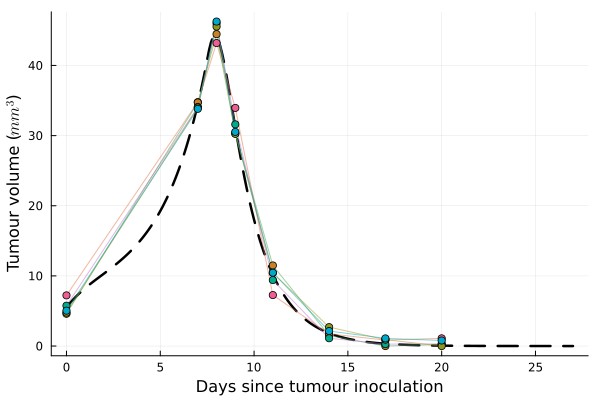
\includegraphics[scale=0.4]{model_validation/fd_1.png}
        \caption{Dataset A}
    \end{subfigure}%
    \begin{subfigure}{.5\linewidth}
        \centering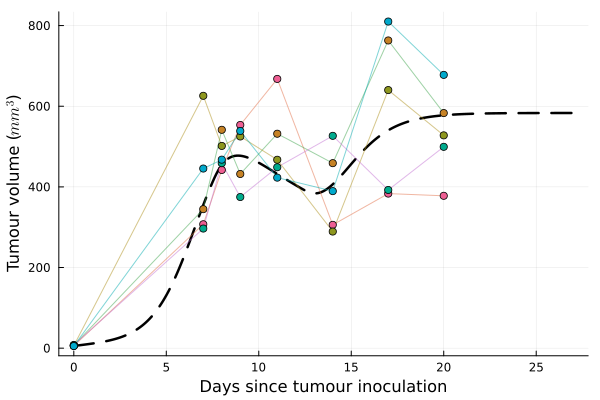
\includegraphics[scale=0.4]{model_validation/fd_2.png}
        \caption{Dataset B}
    \end{subfigure}
    \caption{Plot of the fake data points (colored lines and scatter plot) along with the original growth curve (dashed line)}
    \label{fig:fd_1}
\end{figure}

\textit{Results}\\[5pt] 
Before checking if the estimated values match the true ones, we first assess convergence of the MCMC chains. Th $\hat{R}$ values (see Section~\ref{sec:eval}) are reported in Table.~\ref{tbl:rhat_2} as the average $\hat{R}$ value accross the 3 parameters. It must be noted that often, out of the 5 chains per inference, some chains  get trapped (assessed by visual inspection). In that case, they are excluded from the $\hat{R}$ calculation, and this is reported in the ``Number of Chains'' column. If all chains are exlcuded, meaning that none of them converged, we simply report N/A.

\begin{table}[!h]
    \centering
    \caption{Assessement of convergence for the MCMC chains for uninformative priors (3 free parameters)}
    \begin{tabular}{c|c||c|c|c}
        \hline
        Data set & Pooling Type & $\hat{R}$ diagnostic & Number of Chains & Convergence  \\ \hline 
        \multirow{2}{*}{A}      & None     & 116.08 & N/A & No \\
                                & Complete & 298.67 & N/A & No \\ \hline 
        \multirow{2}{*}{B}      & None     & 1.092  & 3/5 & No \\
                                & Complete & 3.11   & N/A & No \\ \hline 
    \end{tabular}
    \label{tbl:rhat_2}
\end{table}
Looking at Table~\ref{tbl:rhat_2}, we can hence conclude that the chains did not converged, meaning that the model cannot make inference with $\boldsymbol{\theta} \in \mathbb{R}^3$ and uninformative priors. To further diagnose the model, we performed another set of inferences, except that the priors where highly informative:
\begin{align*}
    \ln(k_6) \sim \text{Cauchy}^-(\theta_{k_6}, 1) \\ 
    \ln(d_1) \sim \text{Cauchy}^+(\theta_{d_1}, 1) \\ 
    \ln(s_2) \sim \text{Cauchy}^-(\theta_{s_2}, 1) \\ 
\end{align*} 
where $\theta_x$ represent the true value of parameter $x$. Convergence of this new set of inferences is shown in Table~\ref{tbl:rhat_3}. As we can see, convergence of the MCMC chains are still very poor, even with highly informative priors centered on the true parameter values.
\begin{table}[!h]
    \centering
    \caption{Assessement of convergence for the MCMC chains for uninformative priors (3 free parameters)}
    \begin{tabular}{c|c||c|c|c}
        \hline
        Data set & Pooling Type & $\hat{R}$ diagnostic & Number of Chains & Convergence  \\ \hline 
        \multirow{2}{*}{A}      & None  & 18.15 & N/A & No \\
                                & Complete & 45.96 & N/A & No \\ \hline 
        \multirow{2}{*}{B}      & None  & 1.505 & 3/5 & No \\
                                & Complete & 1.014 & 2/5 & Yes \\ \hline 
    \end{tabular}
    \label{tbl:rhat_3}
\end{table}
\\[12pt]
It might be objected that Cauchy distributions are by definition not too informative since a non-negligible portion of their mass stretches well beyond their standard deviation, contrary to normal distributions. This hence motivated us to perform one last fake data check, using the normal priors shown below to be even more informative: 
\begin{align*}
    \ln(k_6) \sim \mathcal{N}^-(\theta_{k_6}, 0.3) \\ 
    \ln(d_1) \sim \mathcal{N}^+(\theta_{d_1}, 0.3) \\ 
    \ln(s_2) \sim \mathcal{N}^-(\theta_{s_2}, 0.3) \\ 
\end{align*}
Convergence results are shown in Table.~\ref{tbl:rhat_4}. The main result is that chains converged or were close to convergence only for dataset D, showing that a log-normal transformation is key to make exploration of the posterior easier to perform. Whilst the overall convergence rate is still very low given the informative normal priors, this series of fake data checks for the case of three free parameters highlighted the key role of the log-transformation.

\begin{table}[!h]
    \centering
    \caption{Assessement of convergence for the MCMC chains for uninformative priors (3 free parameters)}
    \begin{tabular}{c|c||c|c|c}
        \hline
        Data set & Pooling Type & $\hat{R}$ diagnostic & Number of Chains & Convergence  \\ \hline 
        \multirow{2}{*}{A}      & None     & 7.387 & N/A & No \\
                                & Complete & 39.17 & N/A & No \\ \hline 
        \multirow{2}{*}{B}      & None     & 1.066 & 3/5 & Yes \\
                                & Complete & 1.111 & 5/5 & No \\ \hline 
    \end{tabular}
    \label{tbl:rhat_4}
\end{table}
~\\
\textit{Conclusion}\\[5pt]
Even with informative priors, the MCMC chains do not even converge. This suggests that the likelihood function is too difficult to explore and might contain discontinuities. As suggested by Gelman et al. (2020) in their \textit{Bayesian Workflow} document, the first step to take to address this issue would be to drastically simplify the likelihood function and re-assess performance of the model of fake datasets. Another approach that we are currently exploring would be to use Approximate Bayesian Computation.


\section{Implementation Plan}\label{sec:plan}

\begin{figure}[!ht]
    \centering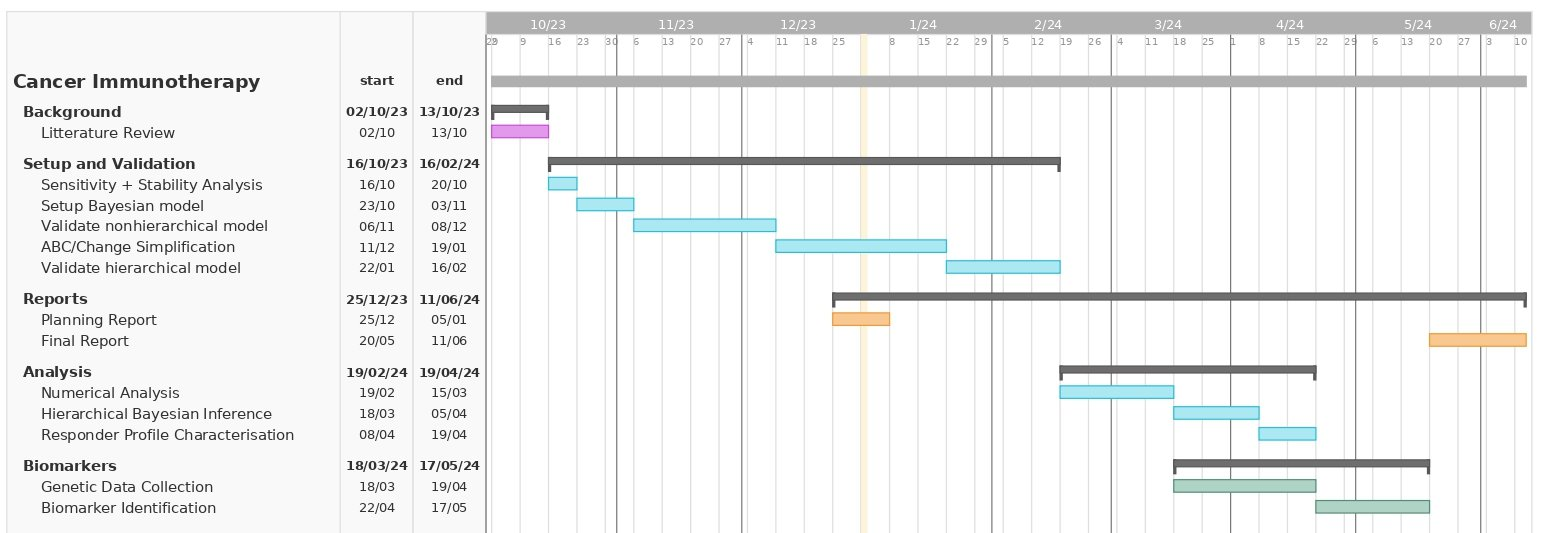
\includegraphics[scale=0.3]{pd.jpg}
\end{figure}

\newpage 
\clearpage
\newpage

\addcontentsline{toc}{section}{References}
\bibliographystyle{unsrt}
\bibliography{biblio}


\end{document} % This is the end of the document

%% Trash-city

% The goal of immunotherapy is to use a specific type of cytotoxic immune cells, the CD8$^+$ cells, to fight against cancer \cite{ReviewCPI}. As cancer can escape these killer cells through various mechanisms, this lead to a range of difference 

% While all cancer immunotherapies focus on using the natural immune system to fight against cancer, many different variations exist. The specific therapy of concern in this project is a combination of cytokine-based treatments and immune checkpoint inhibitors. Before explaining its specificities in more details, we will review the general principles behind the two aforementionned types of immunotherapy. In both case, a specific type of T-lymphocyte, the CD8$^+$ T-cells, is the central actor . CD8$^+$ differentiate itself from other T-cells through the expression of the membrane receptor CD8, and its main function is to directly carry out cytotoxic activity (i.e. killing the malignant cells) after detecting tumoural antigen~\cite{cd8Effects}.
%

% it is a pleiotropic molecule, meaning that it results in the release of numerous cytokines throughout the immune response~\cite{il12CytokineStorm}. One particular molecule released during this cytokine storm is the interferon-$\gamma$ (IFN$\gamma$). IFN$\gamma$ plays a dominant role within this cytokine storm, as not only does it have anti-angiogenesis effect~\cite{ifngAngiogenesis}, thus limiting cancer growth; but it also stimulate production Natural Killer cells \cite{ifngNKProd} (another type of cytotoxic cells capable of attacking tumours) and upregulate antigen-presenting pathways within tumour cells \cite{ifngAntigenExposure}. Finally, IL-12 facilitates T-cell proliferation by reducing negative regulatory pathways that lead to immunosuppression. Indeed, IL-12 inhibts the effect of the immune checkpoint PD-1, similarly to chekpoint inhibitors (CPI) treatments \cite{reducImmunoSuppression}. The more details mode of action is described in the following paragraph. [maybe need to mention trAEs? and poor performance so far...]
%
